\documentclass[11pt,a4paper]{article}
\usepackage[utf8]{inputenc}
\usepackage[T1]{fontenc}
\usepackage{tgpagella}
\usepackage[spanish]{babel}
\usepackage{geometry}
\usepackage{booktabs}
\usepackage{xcolor}
\usepackage{titlesec}
\usepackage{fancyhdr}
\usepackage[parfill]{parskip}
\usepackage[expansion=false]{microtype}
\usepackage{hyperref}
\usepackage{setspace}
\usepackage{needspace}
\usepackage{graphicx}
\widowpenalty=10000
\clubpenalty=10000
\displaywidowpenalty=10000

\geometry{top=3.0cm,bottom=3.0cm,left=3.5cm,right=3.5cm}
\setlength{\parskip}{0.65em}
\setlength{\parindent}{0em}

\definecolor{azulai}{RGB}{30,80,140}
\definecolor{doradoai}{RGB}{140,90,0}
\definecolor{grisai}{RGB}{70,70,70}

\titleformat{\section}{\Large\bfseries\color{azulai}}{}{0em}{}[{\color{azulai}\titlerule[0.5pt]}]
\titlespacing*{\section}{0pt}{1.8em}{0.8em}
\titleformat{\subsection}{\large\bfseries\color{doradoai}}{}{0em}{}
\titlespacing*{\subsection}{0pt}{1.4em}{0.5em}
\titleformat{\subsubsection}{\normalsize\bfseries\color{grisai}}{}{0em}{}
\titlespacing*{\subsubsection}{0pt}{1.0em}{0.3em}

\pagestyle{fancy}\fancyhf{}
\rhead{\textcolor{grisai}{\small Virginia Riezu — Arquitectura Interna}}
\lhead{\textcolor{grisai}{\small Júpiter · Saturno}}
\cfoot{\textcolor{grisai}{\small\thepage}}
\renewcommand{\headrulewidth}{0.3pt}

\hypersetup{colorlinks=true,linkcolor=azulai,urlcolor=azulai}
\setstretch{1.45}
\tolerance=1500
\emergencystretch=4em

\begin{document}

% ── Portada ──────────────────────────────────────────────────────────────────

\begin{titlepage}
\centering

\vspace*{2cm}

{\Huge\bfseries\color{azulai} Júpiter · Saturno}\\[0.4cm]

{\large\color{grisai} Arquitectura Interna}\\[0.25cm]

{\small\itshape\color{grisai}
Crecimiento, estructura y organización interna
}\\[1.8cm]

{\huge\color{doradoai} Virginia Riezu}\\[1.2cm]

{\Large 06/09/1975 \quad 01:30}\\[0.25cm]

{\Large Pamplona, España}\\[0.25cm]

{\normalsize
Lat: 42.8157° \quad
Lon: -1.6522° \quad
UTC+02:00
}\\[0.4cm]

{\normalsize
Ascendente: Géminis 29°04'
\quad
MC: Piscis 3°22'
}\\[1.6cm]

\begin{tabular}{ll}
\textbf{Júpiter:} & Aries — Casa 11 23°54' (Retrógrado) \\
\textbf{Saturno:} & Cáncer — Casa 2 28°53' \\
\end{tabular}

\vfill

{\small\color{grisai}
Generado el 20/05/2026
}

\end{titlepage}

	ableofcontents
space{0.8cm}

% ── Datos de referencia ──────────────────────────────────────────────────────

\section{Datos de referencia}

\begin{center}
\begin{tabular}{llll}
\toprule
\textbf{Punto} & \textbf{Signo} & \textbf{Casa} & \textbf{Posición} \\
\midrule

Júpiter (Retrógrado) &
Aries &
Casa 11 &
23°54' \\

Saturno &
Cáncer &
Casa 2 &
28°53' \\

Sol &
Virgo &
Casa 4 &
12°46' \\

Luna &
Virgo &
Casa 4 &
15°17' \\

Mercurio &
Libra &
Casa 5 &
8°18' \\

Venus &
Leo &
Casa 3 &
28°18' \\

Marte &
Géminis &
Casa 12 &
12°51' \\

Urano &
Libra &
Casa 5 &
29°54' \\

Ascendente &
Géminis &
--- &
29°04' \\

Medio Cielo &
Piscis &
--- &
3°22' \\

\bottomrule
\end{tabular}
\end{center}

\vspace{0.8cm}

\subsection*{Aspectos entre funciones}

\begin{center}
\begin{tabular}{lllll}
  \toprule
  \textbf{Planeta 1} & \textbf{Asp.} & \textbf{Planeta 2} & \textbf{Tipo} & \textbf{Orbe} \\
  \midrule
  Saturno & cua & Urano & Cuadratura & 1.0° \\
  Júpiter & conj & Quirón & Conjunción & 1.6° \\
  Saturno & cua & Quirón & Cuadratura & 3.4° \\
  Júpiter & tri & Venus & Trígono & 4.4° \\
  Júpiter & cua & Saturno & Cuadratura & 5.0° \\
  Júpiter & opo & Urano & Oposición & 6.0° \\
  \bottomrule
\end{tabular}
\end{center}

\vspace{1cm}

\begin{center}
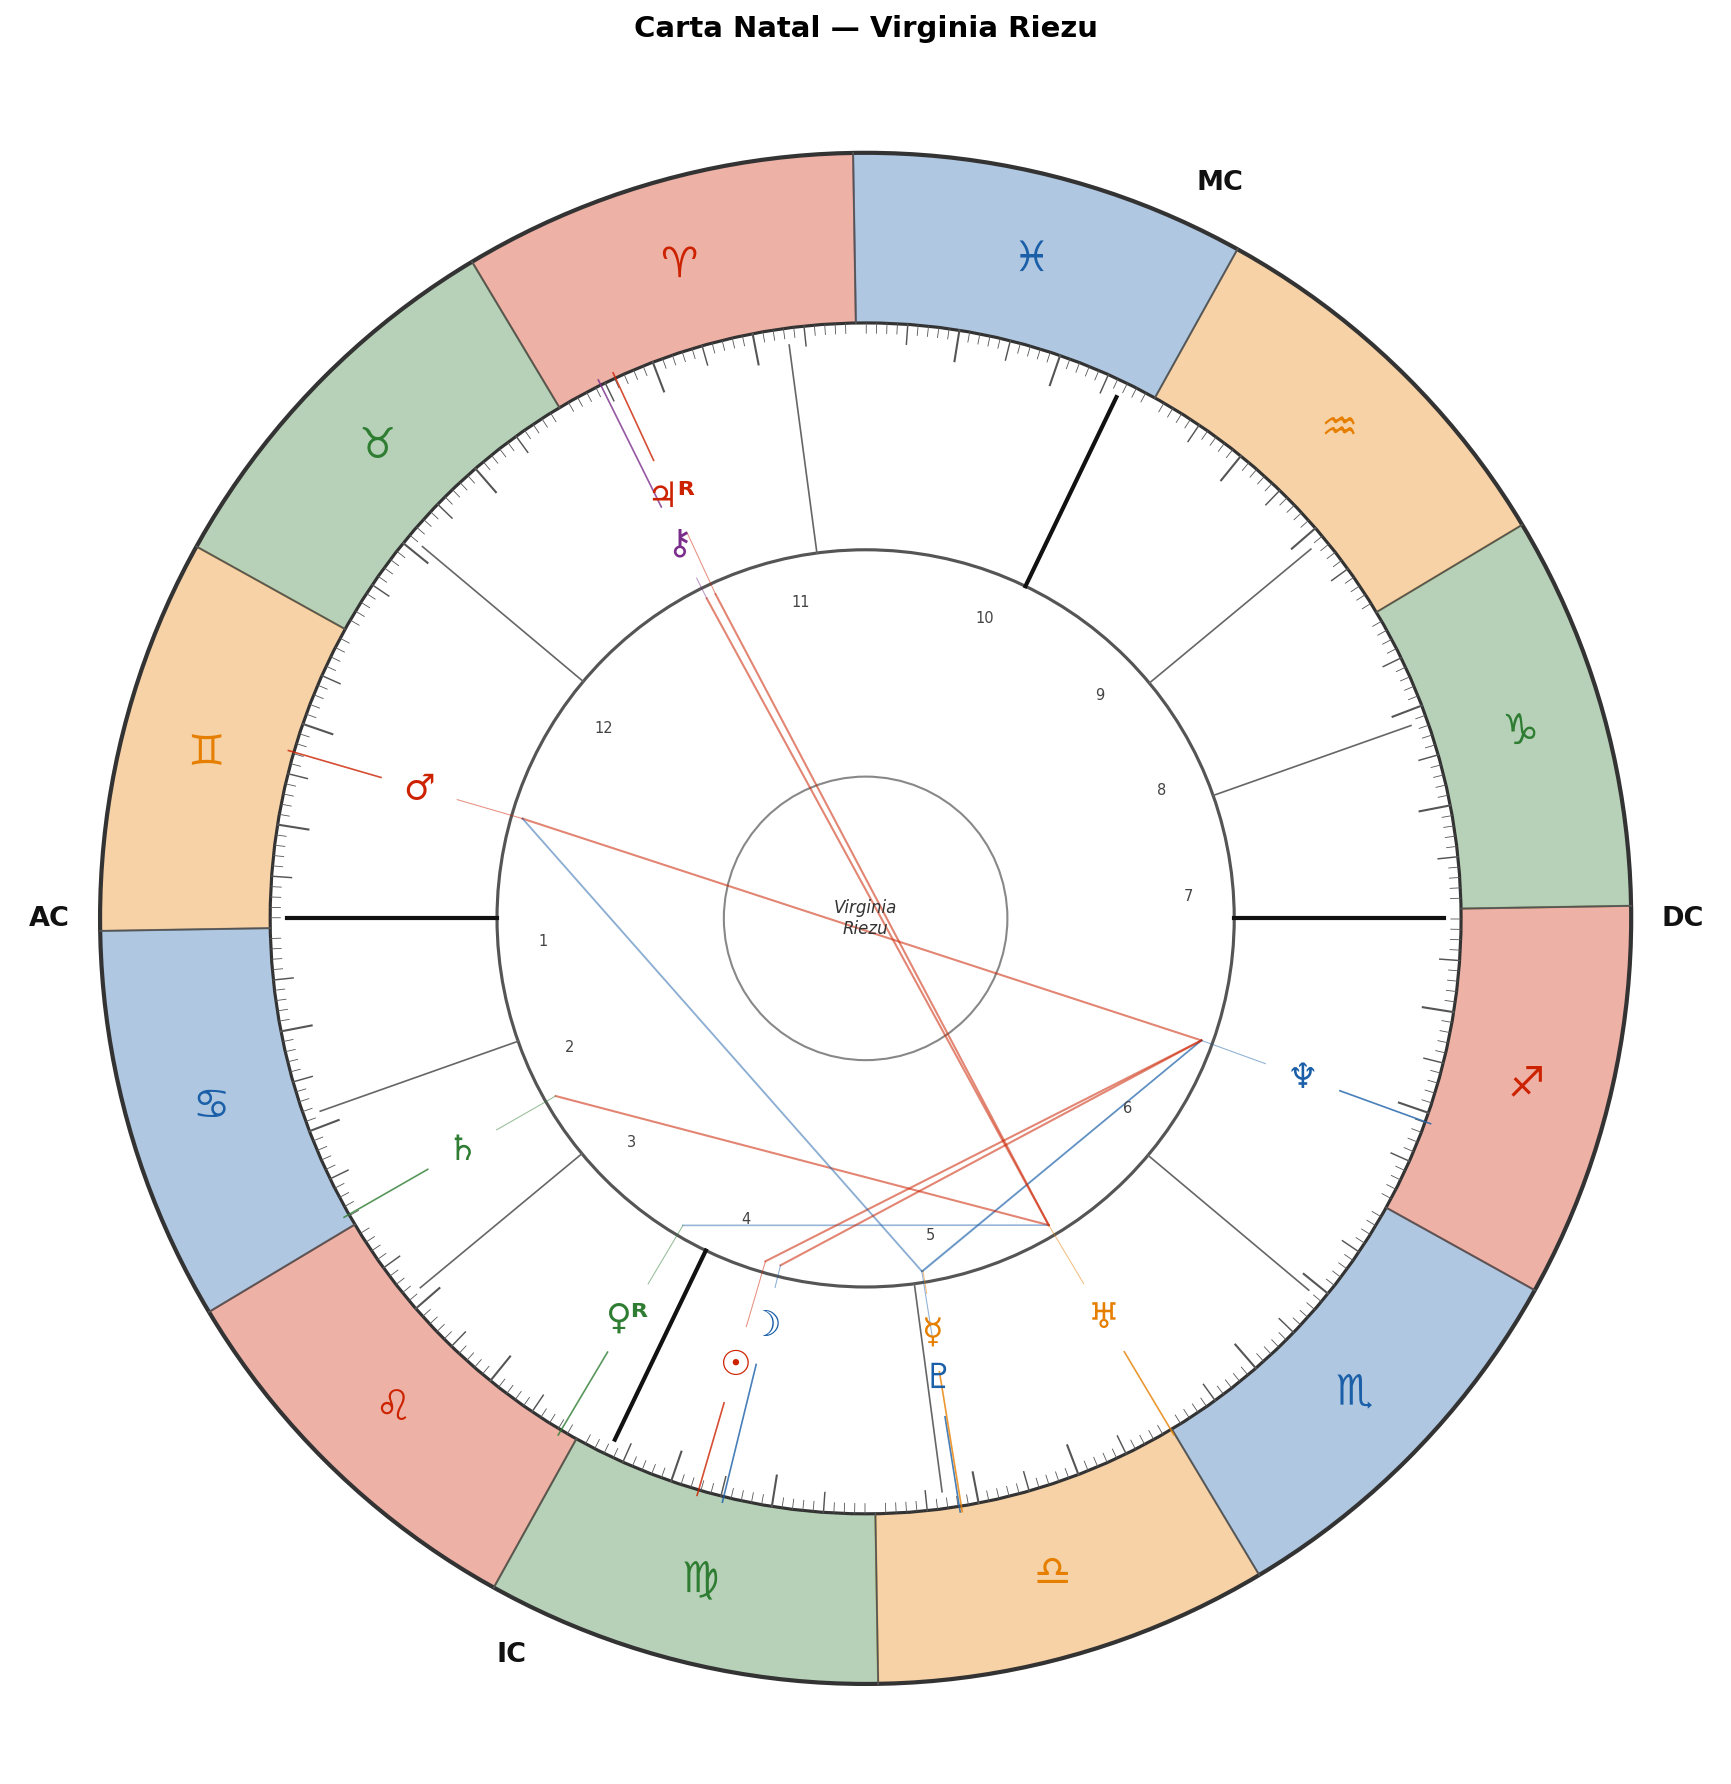
\includegraphics[width=0.72\textwidth]{Virginia_Riezu_rueda.png}
\end{center}

\vspace{0.8cm}
\Needspace{5\baselineskip}


% ── Interpretación ───────────────────────────────────────────────────────────

\section{Interpretación — Arquitectura Interna}

\begin{center}
{\small\itshape
No se trata de definir quién eres.\\
Se trata de observar cómo tiendes a crecer, estructurarte\\
y sostener tu relación con el mundo.
}
\end{center}

\vspace{0.8cm}
\Needspace{5\baselineskip}

% ── 1. Estructura general ────────────────────────────────────────────────────

\subsection{1. Estructura general}

Júpiter está en Aries, Casa 11: muestra cómo tiendes a crecer, abrir posibilidades y ampliar tu relación con el mundo.
Saturno está en Cáncer, Casa 2: muestra cómo tiendes a estructurarte, sostener límites y construir estabilidad.

Expansión (Aries, Fuego) y estructura (Cáncer, Agua) operan en elementos que crean tensión. Puede haber momentos en los que crecer y sostenerte requieran movimientos internos diferentes, por lo que la integración necesita más atención consciente.

Aspectos relevantes: Júpiter–Saturno en cuadratura (orbe 4.98°), Júpiter–Venus en trígono (orbe 4.41°), Júpiter–Urano en oposición (orbe 5.99°), Saturno–Urano en cuadratura (orbe 1.01°).

\vspace{0.8cm}
\Needspace{5\baselineskip}

% ── 2. Júpiter ───────────────────────────────────────────────────────────────

\subsection{2. Júpiter — Expansión y crecimiento}

\subsubsection*{
Júpiter en Aries
— Casa 11 (Retrógrado)
}

Tiendes a crecer a través de la iniciativa, el movimiento y la exploración de territorio nuevo. La expansión aparece cuando puedes empezar algo, abrir camino o avanzar hacia lo desconocido. Necesitas sentir impulso, dirección y margen de acción para que la energía de crecimiento se active.

En situaciones de desbordamiento: puedes abrir más frentes de los que realmente puedes sostener. La energía se dispersa entre comienzos, impulsos o proyectos que no siempre llegan a consolidarse. En momentos de estancamiento: necesitas demasiado estímulo, reto o sensación de avance para mantenerte en movimiento. Si no hay una dirección clara hacia la que ir, puede aparecer actividad constante sin sensación real de crecimiento.

Tiendes a crecer a través de grupos, redes y proyectos compartidos. La expansión aparece cuando puedes participar en algo colectivo y aportar tu visión a espacios más amplios que lo estrictamente personal. Necesitas conexión con ideas, personas o proyectos que miren hacia el futuro.

Júpiter está retrógrado. El crecimiento tiende a desarrollarse de forma más interna y menos visible externamente al principio. Puedes necesitar más tiempo para traducir expansión o comprensión en movimientos concretos hacia fuera.

\vspace{0.8cm}
\Needspace{5\baselineskip}

% ── 3. Saturno ───────────────────────────────────────────────────────────────

\subsection{3. Saturno — Estructura y sostén}

\subsubsection*{
Saturno en Cáncer
— Casa 2
}

Tiendes a estructurarte a través de la protección emocional y la construcción de espacios seguros. Necesitas sentir contención, intimidad y cierto resguardo para sostenerte de forma estable. La estructura aparece delimitando qué puedes sostener emocionalmente y qué no.

El límite aparece en la cantidad de carga emocional que puedes absorber antes de saturarte. No todo puede entrar dentro de tu espacio interno.

Cuando la estructura deja de sostenerse: puedes cerrarte defensivamente o reaccionar desde la protección. La necesidad de resguardo sustituye la capacidad de procesar lo que ocurre.

Tiendes a estructurarte a través de los recursos, la estabilidad y la gestión de lo que tiene valor para ti. La seguridad suele construirse lentamente, mediante constancia y acumulación progresiva. Necesitas sentir que existe una base concreta sobre la que apoyarte.

El límite aparece cuando intentas sostener más de lo que tus recursos reales permiten. La estabilidad depende de la capacidad de administrar energía, tiempo y recursos de forma sostenible.

\vspace{0.8cm}
\Needspace{5\baselineskip}

% ── 4. Integración ───────────────────────────────────────────────────────────

\subsection{4. Integración — Crecimiento y estructura}

Júpiter cuadratura Saturno: crecimiento y estructura están en tensión constante. Puedes sentir que una parte de ti quiere ampliar, probar o abrir posibilidades mientras otra necesita controlar, contener o limitar el movimiento.

A veces puedes expandirte más allá de lo que realmente puedes sostener; otras veces puedes frenarte demasiado antes de permitirte crecer. El trabajo suele estar en reconocer cuándo estás en cada extremo.

Cuando Júpiter domina: puedes iniciar más de lo que realmente puedes sostener, dispersando energía en varios frentes sin completar ninguno. La estructura de Saturno en Cáncer no compensa con suficiente rapidez y lo que ganas en amplitud empieza a perder forma.

Cuando Saturno domina: la contención puede suprimir lo que necesita circular, y lo no expresado se acumula. La expansión de Júpiter en Aries no encuentra espacio para activarse y puedes mantener lo que ya existe sin crecer hacia lo que sería posible.

Bajo presión suele aparecer una secuencia bastante reconocible. Primero, Saturno en Cáncer empieza a ceder: los límites emocionales se diluyen y deja de existir suficiente contención. Después, Júpiter en Aries ocupa ese espacio: abres múltiples direcciones al mismo tiempo sin terminar de consolidar ninguna. Desde ahí puedes intentar recuperar estabilidad rápidamente, pero lo que construyes en ese estado suele ser más rígido, reactivo o agotador de sostener. Si el patrón no se reconoce a tiempo, el ciclo tiende a repetirse.

\vspace{0.8cm}
\Needspace{5\baselineskip}

% ── 5. Orientación práctica ──────────────────────────────────────────────────

\subsection{5. Orientación práctica}

\subsubsection*{Desde dónde empezar}

El punto de entrada más accesible suele estar en la expansión (Aries, Casa 11). De las dos funciones, esta requiere menos resistencia para activarse. La forma más natural de empezar es activar movimiento antes de tener todo completamente resuelto. Cuando todo parece bloqueado, comenzar por aquí suele facilitar que la otra función también pueda ponerse en marcha.

\subsubsection*{Qué sostener}

Lo más importante de sostener aparece en Saturno (Cáncer, Casa 2). Bajo presión puedes abrir posibilidades o reaccionar antes de mantener forma estable. Conviene cuidar especialmente mantener límites emocionales suficientes para no saturarte. Muchas veces la primera señal de desgaste aparece cuando sigues haciendo cosas, pero ya no existe suficiente estructura para sostenerlas bien.

\subsubsection*{Qué evitar}

Conviene evitar alternar entre abrir posibilidades sin sostén y sostener estructura sin permitir crecimiento. Con Júpiter–Saturno en cuadratura, crecimiento y estructura no siempre pueden sostenerse al mismo nivel de intensidad al mismo tiempo. Suele ayudar más reconocer qué necesita atención en cada momento que intentar mantener equilibrio constante en todo.

\subsubsection*{Si no se integra}

Cuando crecimiento y estructura dejan de colaborar, puede aparecer expansión sin suficiente sostén o estabilidad sin movimiento real. En ambos casos se pierde parte de lo que realmente podría desarrollarse si ambas funciones trabajaran en la misma dirección.

\subsubsection*{Señal temprana}

La primera señal suele aparecer en Saturno (Cáncer): los límites emocionales dejan de contener suficientemente. Cuando eso ocurre, Júpiter (Aries) tiende a ocupar rápidamente el espacio disponible y la expansión puede acelerarse más de lo que realmente puedes sostener. Detectar la señal temprano suele evitar entrar en ciclos más agotadores.

\vfill

\begin{center}
{\small\itshape\color{grisai}
La astrología se utiliza aquí como herramienta simbólica de observación\\
y no como una definición cerrada de la persona.
}
\end{center}

\end{document}
